\begin{figure}[H]
\centering
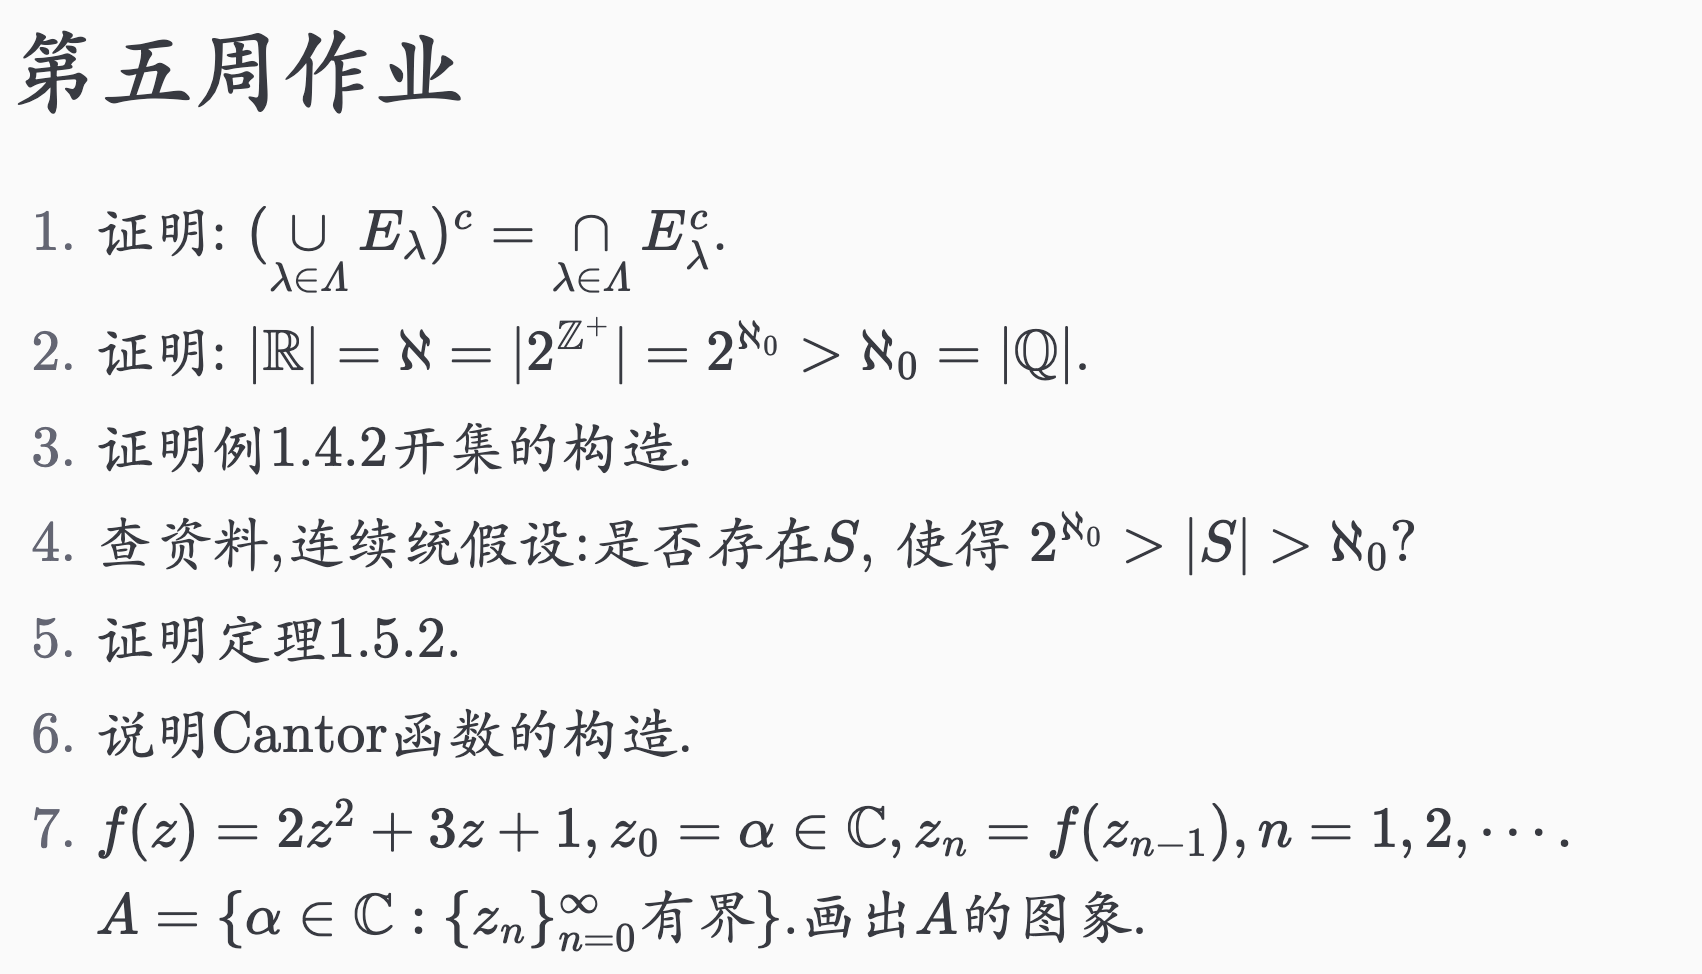
\includegraphics[width=\textwidth]{274eb25c47848157ef9ff45de6f4d76.png}
% \caption{}
\label{}
\end{figure}

\begin{figure}[H]
\centering

\includegraphics[width=\textwidth]{hw5-2025033023.png}
% \caption{}
\label{}
\end{figure}
\begin{proof}
For any $x\in\left( \bigcup_{\lambda\in\Lambda}E_{\lambda} \right)^{c}$, $x\centernot{\in}E_{\lambda},\forall\lambda\in\Lambda$. Thus $x\in \bigcap_{\lambda\in\Lambda}E_{\lambda}^{c}$. For any $x\in \bigcap_{\lambda\in\Lambda}E_{\lambda}^{c}$, then $x\centernot{\in}E_{\lambda},\forall\lambda\in\Lambda$. Then $x\centernot{\in}\bigcup_{\lambda\in\Lambda}E_{\lambda}$, thus $x\in \left( \bigcup_{\lambda\in\Lambda}E_{\lambda} \right)^{c}$. Hence $\left( \bigcup_{\lambda\in\Lambda}E_{\lambda} \right)^{c}=\bigcap_{\lambda\in\Lambda}E_{\lambda}^{c}$.
\end{proof}
\begin{figure}[H]
\centering
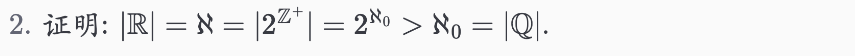
\includegraphics[width=\textwidth]{1-hw5-2025033023.png}
% \caption{}
\label{}
\end{figure}

\begin{theorem}[theorem 2.14 in baby rudin]
Let $A$ be the set of all sequences whose elements are the digits $0$ and $1$. This set $A$ is uncountable.
The elements of $A$ are sequences like $1,0,0,1,0,1,1,1,\dots$
\end{theorem}
Let $E$ be a countable subset of $A$, and let $E$ consist of the sequences $s_1,s_2,s_3,\dots$. We construct a sequence $s$ as follows. If the $n$ th digit in $s_n$ is $1$, we let the $n$ th digit of $s$ be $0$, and vice versa. \textbf{Then the sequence $s$ differs from every member of $E$ in at least one place}; hence $s\not\in E$. But clearly $s\in A$, so that $E$ is a proper subset of $A$.

We have shown that every countable subset of $A$ is a proper subset of $A$. It follows that $A$ is uncountable (for otherwise $A$ would be a proper subset of $A$, which is absurd).

Therefore, $2^{\aleph_0}>\aleph_0$.

\begin{figure}[H]
\centering
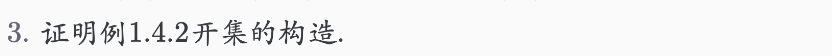
\includegraphics[width=\textwidth]{2-hw5-2025033023.png}
% \caption{}
\label{}
\end{figure}

\begin{figure}[H]
\centering
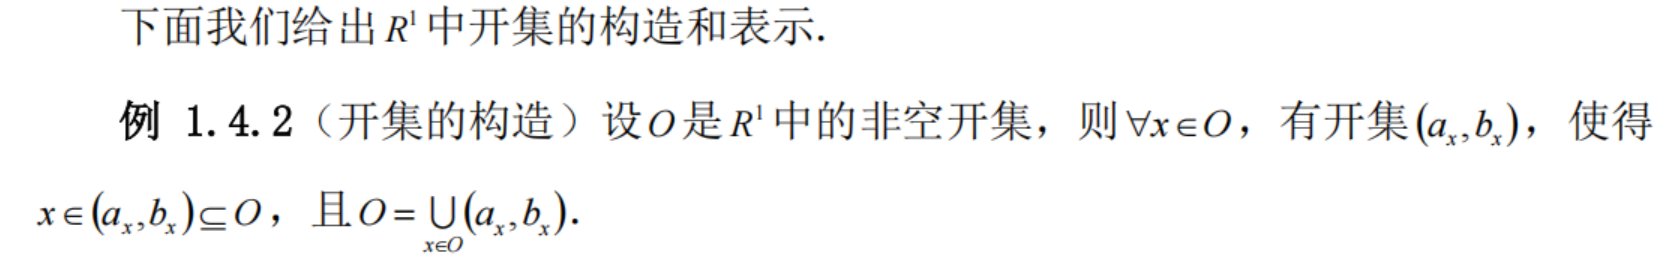
\includegraphics[width=\textwidth]{7-hw5-2025033023.png}
% \caption{}
\label{}
\end{figure}

\begin{proof}
采用蔓延的思想,对于任意 $x\in O$,考虑 $(a_{x},b_{x})\subseteq O$,记
\[
\overline{b_{x}}=\sup \{ b:(a_{x},b)\subseteq O \}\qquad \overline{a_{x}}=\inf \{ a:(a,b_{x})\subseteq O \}
\]
显然 $\overline{b_{x}}\geq b_{x},\overline{a_{x}}\leq a_{x}$. 这里 $a_{x}$ 可能为 $-\infty$,$b_{x}$ 可能为 $+\infty$. 显然区间 $(\overline{a_{x}},\overline{b_{x}})\subseteq O$. 并且 $O\setminus(\overline{a_{x}},\overline{b_{x}})$ 为开集,这是因为对于任意 $x'\in O\setminus(\overline{a_{x}},\overline{b_{x}})$,存在 $I_{x'}\subseteq O$,若 $I_{x'}\cap(\overline{a_{x}},\overline{b_{x}})\neq \varnothing$,这与 $\overline{a_{x}},\overline{b_{x}}$ 定义矛盾!故 $I_{x'}\subseteq O\setminus(\overline{a_{x}},\overline{b_{x}})$.

存在如下映射
\[
O\overset{ f }{ \to } \{ (\overline{a_{x}},\overline{b_{x}}):x\in O \}\overset{ g }{ \to } \mathbb{Q}\qquad x\mapsto(\overline{a_{x}},\overline{b_{x}})\mapsto r_{x}\in(\overline{a_{x}},\overline{b_{x}})
\]
显然 $g$ 是单射,因此 $\#\{ (\overline{a_{x}},\overline{b_{x}}):x\in O \}\leq\#\mathbb{Q}=\aleph_0$.
\end{proof}

\begin{figure}[H]
\centering

\includegraphics[width=\textwidth]{3-hw5-2025033023.png}
% \caption{}
\label{}
\end{figure}

不存在

\begin{figure}[H]
\centering
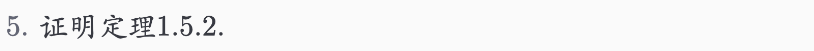
\includegraphics[width=\textwidth]{4-hw5-2025033023.png}
% \caption{}
\label{}
\end{figure}

\begin{figure}[H]
\centering
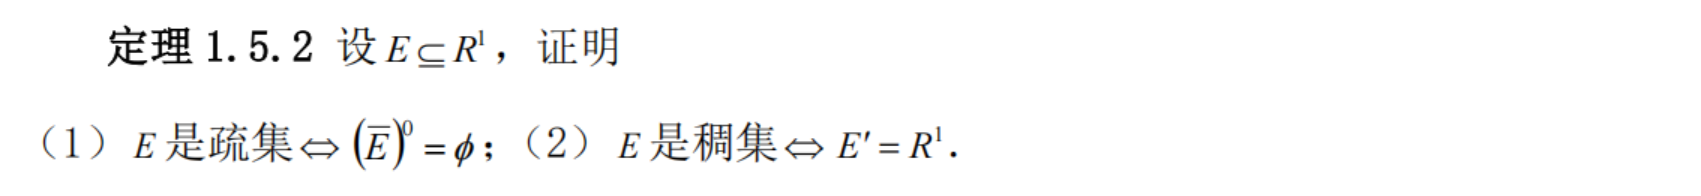
\includegraphics[width=\textwidth]{hw5-2025033100.png}
% \caption{}
\label{}
\end{figure}

(1) 若 $(\overline{E})^{\circ}=\varnothing$, 则 $\forall x\in \overline{E}$,$x$ 不是 $\overline{E}$ 的内点,也就是说 $x$ 的“附近”不包含于 $\overline{E}$ 中. 对于任意充分小的 $\epsilon>0$,$(x-\epsilon, x+\epsilon)\cap \overline{E}=\{ x \}$. 由疏集的定义,对于 $\mathbb{R}$ 中的任意非空开集 $G$,若 $x\in E\cap G$,那么存在 $\delta$ 使得 $(x-\delta,x+\delta)\subseteq G$,存在 $(x-\epsilon,x+\epsilon)\cap \overline{E}=\{ x \}$,选取 $G$ 的子集 $(x,x+\min\{ \epsilon,\delta \})$,这个集合与 $E$ 不相交,因此 $E$ 是疏集.

若 $E$ 是疏集,但 $(\overline{E})^{\circ}\neq\varnothing$. 那么存在 $x\in \overline{E}$,使得存在 $(x-\epsilon,x+\epsilon)\subseteq \overline{E}$. 选取区间 $(x-\epsilon/2,x+\epsilon/2)$,那么它有非空开子集 $I_{x}$ 与 $E$ 不相交,这不可能发生在 $\mathbb{R}^{1}$ 的拓扑上!

因此,$E$ 是疏集等价于 $(\overline{E})^{\circ}=\varnothing$.

(2) 这是显然的.

\begin{figure}[H]
\centering
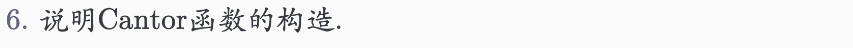
\includegraphics[width=\textwidth]{5-hw5-2025033023.png}
% \caption{}
\label{}
\end{figure}

\begin{figure}[H]
\centering
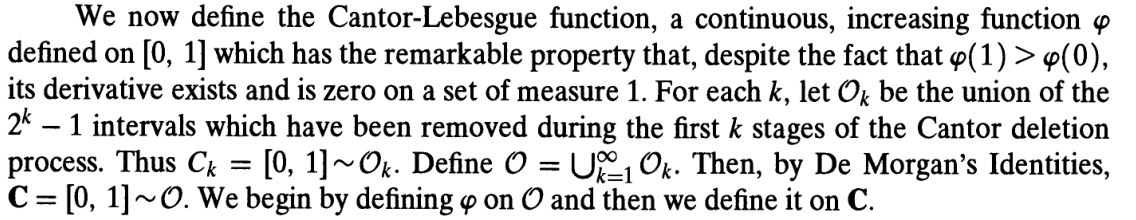
\includegraphics[width=\textwidth]{1-hw5-2025033100.png}
% \caption{}
\label{}
\end{figure}
\begin{figure}[H]
\centering
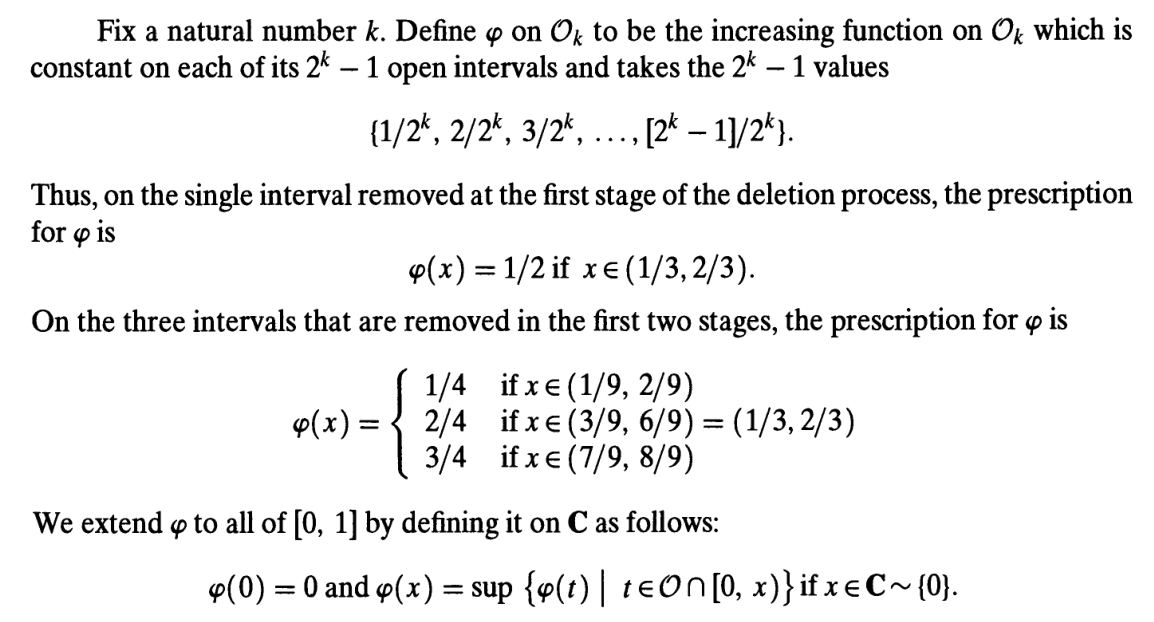
\includegraphics[width=\textwidth]{2-hw5-2025033100.png}
% \caption{}
\label{}
\end{figure}

\begin{figure}[H]
\centering
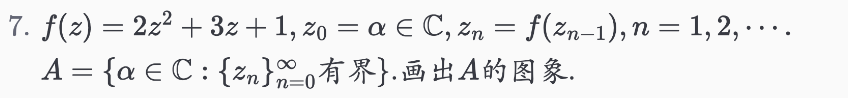
\includegraphics[width=\textwidth]{6-hw5-2025033023.png}
% \caption{}
\label{}
\end{figure}

$A$ is a Julia set.

\begin{lstlisting}[language=mathematica]
JuliaSetPlot[2  z^2 + 3  z + 1, z, ColorFunction -> None]
\end{lstlisting}
\begin{figure}[H]
\centering
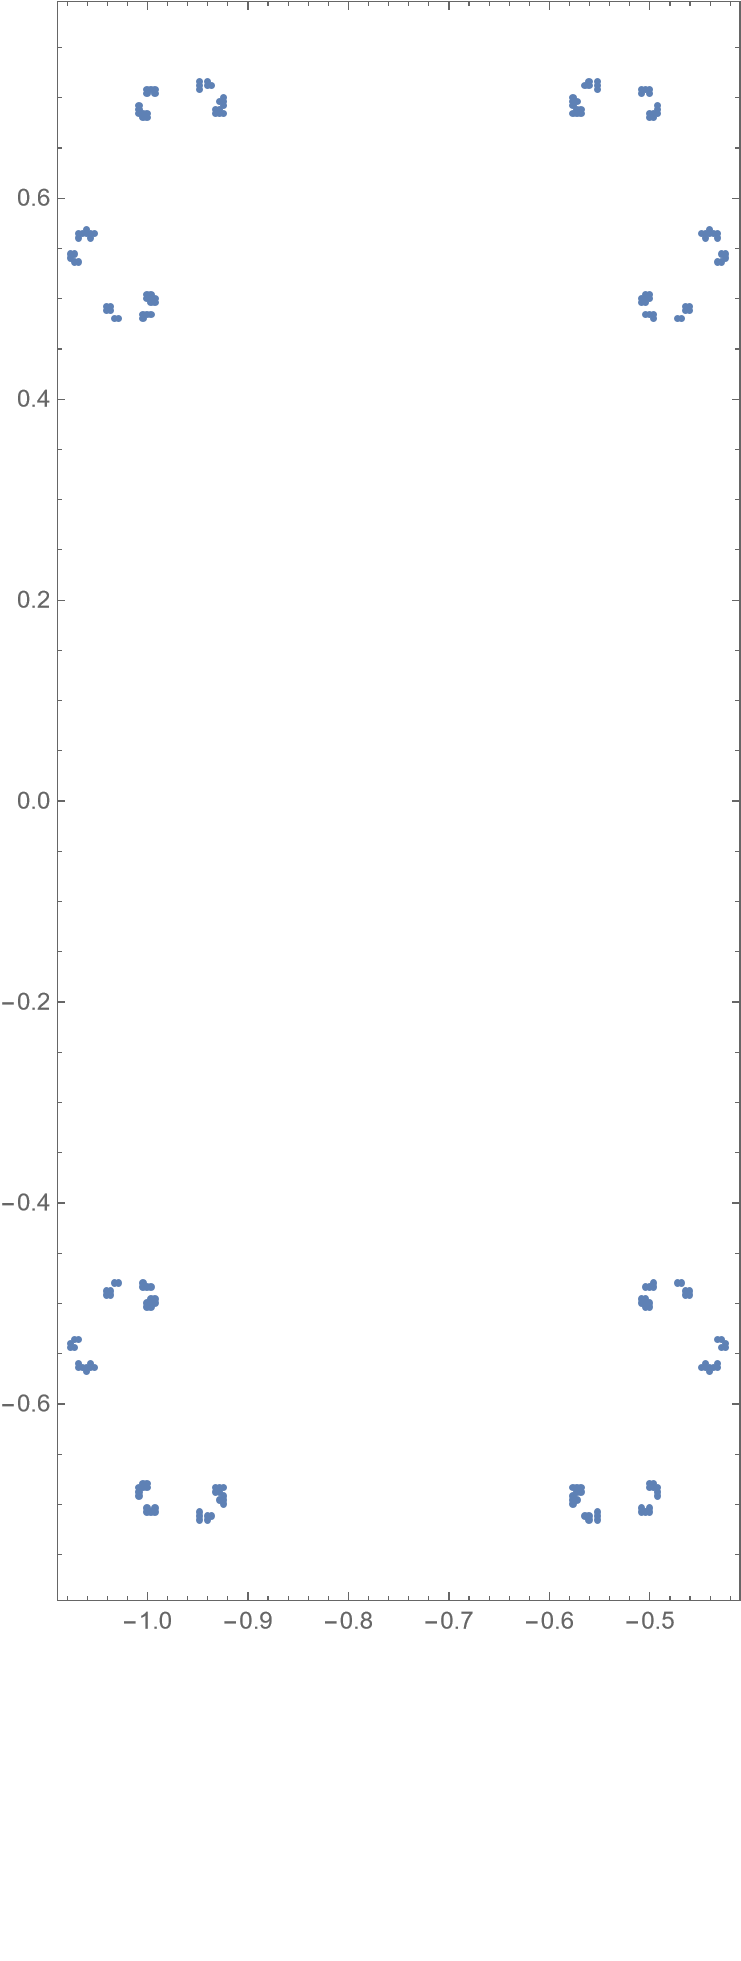
\includegraphics[width=\textwidth]{1-hw5-2025040218.png}
% \caption{}
\label{}
\end{figure}
